\chapter{Two different appoaches to compute the boundaries in target phase space}\label{chap:triangulation}
\section{The $\alpha$-shapes approach}

Given a finite set $\mathcal{S} $ of points we want to determine the shape formed by these points. $\alpha$-shapes are geometrical objects which give  us a good approximation of the shape of a given point set $\mathcal{S}$. Before giving a formal definition we explain an intuitive interpretation of $\alpha$-shapes. As mentioned in \cite{edelsbrunner1994three}
we can think of  an $\alpha$-shape as a mass of ice-cream with several chocolate pieces. The mass making up the space $\mathbb{R}^3$ and the chocolate pieces are the point set $\mathcal{S}$. Then the aim is to find the shape formed by the chocolate pieces. We can use a spoon with a spherical shape and carve out all parts of the ice-cream without removing the chocolate pieces. We will obtain a shape formed by arcs and points (see figure below for the two-dimensional case).
\begin{figure}[htbp]
\begin{center}
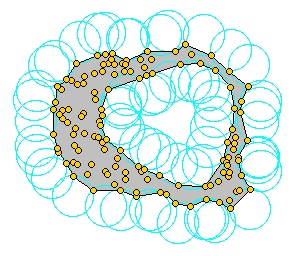
\includegraphics[width=7cm]{shape.jpg}
\label{fig:shape}
\caption{Construction of $\alpha$-shape given a set of points in $\mathbb{R}^2$.}
\end{center}
\end{figure}
Straightening the arcs to triangles and line segments we have an intuitive description of what is called the $\alpha$-shape of $\mathcal{S}$. In our example, the parameter $\alpha$ determines of the radius of the carving spoon. If $\alpha$ is equal to $0$ the shape degenerates to the point set $\mathcal{S}$. On the other hand, when $\alpha\rightarrow\infty$ the $\alpha$-shape is simple the convex hull.
More precisely the process is summarized as follows.
Given a point cloud $\mathcal{S}$ we start with a triangulation of it (a possible choice could be the Delaunay triangulation described in the next section). For each triangle we calculate the radius of the circumcircle. If the radius is larger that $\alpha$ the triangle is removed from the shape. The rule of the parameter $\alpha$ is highly significant in this procedure. Hence we have to choose it in such a way to get a better approximation. The choice of the parameter $\alpha$ is closely related to the radius of the circumcircles. A possible strategy is to find the radius of the greater empty circumcircle. Thus $\alpha$ is related to the density of the points. In particular we have:
\begin{equation}
\alpha=C\frac{1}{\Delta}\;,
\end{equation}
with $C$ a constant that can be determined by a simulation and $\Delta$ the density of the point set $\mathcal{S}$ defined as:
\begin{equation}
\Delta=\frac{N}{\mbox{surface area}}\; ,
\end{equation}
where $ N $ is the number of points in $\mathcal{S}$ and the surface area is the area inside the boundaries of the region formed by the points cloud. Hence $\Delta$ is a constant.
As mentioned above to find the $\alpha$-shape of a point cloud we need a triangulation and a possible choise could be the Delaunay triangulation.
As explained in \cite{portegies2013fast} we can see a Delaunay triangulation as the dual of a Voronoi diagram.
Let us define a Voronoi diagram in a metric space.
\begin{defn}
Let $X$ be a space endowed with a distance $\textrm{d}$ and $\mathcal{S}=\{S_1,\cdots,S_n\}$ a set formed by subsets of $X$. The Voronoi cell $R_k$ associated with the set $S_k$ where $k\in\{1,\cdots,n\}$ is defined as follows:
\begin{equation}
R_k=\{\textbf{x}\in X\; | \;\textrm{d}(\textbf{x},S_k)\leq \textrm{d}(\textbf{x},S_j) \quad \forall j\neq k \}\,,
\end{equation}
where $\textrm{d}(x,A)=\inf \{\textrm{d}(x,a)\; | a\in A\} $.
The Voronoi diagram is defined as the tuple of the cells $(R_k)_{k\in\{1,\dots,n\}}$ that are assumed to be disjoint.
\end{defn}
The simplest case that we can have is the two-dimensional case that is the case where $X=\mathbb{R}^2$.
The tuple $\mathcal{S}=\{1,\cdots,n\}\subset \mathbb{R}^2$ is now a set of points. The Voronoi diagram of $\mathcal{S}$ is a subsection of $\mathbb{R}^2$ such that every other region around a point $p\in \mathcal{S}$ contains all points that are closer to $p$ than to every point in $\mathcal{S}$. A triangulation of the point set $\mathcal{S}$ is a set of edges $\mathcal{E}$ whose extremes are points of $\mathcal{S}$ such that the faces of each triangle are bounded by three edges and any edge that is not in $\mathcal{E}$ intersects one of the existing edges. The Delaunay triangulation is the dual graph of the Voronoi diagram: it consists of vertices (the points in $\mathcal{S}$) and it has an edge between two vertices if the two corresponding faces share an edge. \\
The Delaunay triangulation triangulates the convex hull of the point set $\mathcal{S}$. Instead, the $\alpha$-shape of a point set is formed only by the triangles (taken from the Delaunay triangulation) that satisfy the "$\alpha$-test" and therefore is a suitable method to reconstruct the surface formed by a point cloud.
Even if $\alpha$-shapes are a powerful tool to reconstruct surfaces, some simulations show that there exist surfaces that are not described well by $ \alpha $-shapes. Indeed for some particular surface there exist no value of $\alpha$ that includes all desired triangles and deletes all undesired triangles. For instance, since the parameter $\alpha$ depends on the density of the point cloud, is intuitively clear that using $\alpha$-shapes for a non-uniform points set we won't get a good approximation of the surface. Furthermore, the $\alpha$-shape method doesn't work well when there is a sharp turn or a joint. In this case $\alpha$-shapes often give a "webbed-foot" appearance at such joints since they improperly connect the adjacent surfaces. Hence a generalization of "classical" $\alpha$-shapes is required. In the next section a method to solve the "density problem" for two separated and close objects is described.
In \cite{teichmann1998surface} Teichmann and Capps present "Density-scaled $\alpha$-shapes".
The first step of this method is to make a triangulation of the point cloud.
Then the key idea is to compute somehow the point-density of each point and use this to get an approximation of the point density of a triangle. In this way one can reduce the $\alpha$-value in areas where the triangle's point density (see equation \ref{delta_t} for the definition) is higher than average in such a way that is possible to obtain a finer level of detail for areas that have an higher density.
More precisely, each point $ \textbf{p}\in \mathcal{S} $ has a local point density defined as
\begin{equation}
\delta (\textbf{p})= \sum_{\textbf{q}\in \mathcal{S}}\Big( 1-\frac{\textrm{d}(q,p)}{\lambda}\Big) \qquad \forall \textbf{q} \mbox{\;\;such that\;\;} \textrm{d}(\textbf{p},\textbf{q})<\lambda\,,
\end{equation}
where $ \lambda $ is the constant radius of the local neighborhood and $\textrm{d}(\textbf{x},\textbf{y})$ is the Euclidean distance.
When local density is larger than the average, that is when
\begin{equation}
\delta (\textbf{p}) >\frac{1}{| \mathcal{S} |}\sum_{\textbf{q}\in \mathcal{S}}\delta (\textbf{q})
\end{equation}
we know some properties about the region surrounding $\textbf{p}$.
For instance, if the point set is uniformly distributed then it is possible to find areas with a high-density in the case where there are two closely separated surfaces.  In point sets of non-uniform distribution, high densities are found when the surface presents a joint discontinuity. The algorithm developed by Teichmann and Capps is structured as follow.
After computing density information for each point they make a triangulation of the point set. Then they calculate the average density  $\delta(t)$ for each triangle $\Delta_{abc}$ defined as:
\begin{equation}
\delta(t)=\frac{\delta(a)+\delta(b)+\delta(c)}{3 \mu}\,,
\label{delta_t}
\end{equation}
where $\mu$ is the global average density of the entire point set $\mathcal{S}$.
If $\delta(t)$ is greater than $1$ the density of the point cloud is higher. Hence is necessary to define another value of $\alpha$:
\begin{equation}
\alpha^{\;\prime} = \frac{\alpha}{\delta(t)^\sigma}
\end{equation} where $\sigma$ is a value that is adjusted by the user.
If  $\delta$ is less than $1$ the $\alpha$-value is not modified.
In this way it is possible to have a finer precision on the shape formed by the point set where the density is higher than the average density. Hence it is possible to distinguish two separated objects with different density.
\section{The two-faceted cup}
\section{Results for a TIR collimator}
\section{The triangulation refinement approach}
\section{The two-faceted cup}
\section{Results for a TIR collimator}
\section{Results for a Parabolic reflector}
\section{Results for the Compound Parabolic Concentrator (CPC)}
